\chapter{覆盖率引导的多智能体模糊驱动生成系统MAGIC4FDG的需求分析与概要设计}

在进入实现之前，需要先将系统的需求和架构梳理清楚。本章分三部分展开：先通过流程图给出系统运行的全貌，再做需求分析明确系统该做什么、做到什么程度，最后用"4+1"视图把架构设计讲清楚。

\section{系统整体概述}

前面提到，现有LLM驱动生成方法的几个痛点（反馈粒度粗、单模型过载、缺乏知识积累、策略单一），归根结底是把太多事情交给了一个模型。本文的解决思路是将任务拆分，让不同的智能体各司其职，通过共享状态协调，形成"知识提取→策略规划→代码生成→编译修复→模糊测试与覆盖率收集→状态持久化→缺口诊断"的闭环。整个系统由七个节点组成有向无环图，其中四个（Planner、Generation、Patching、Analyst）调用大语言模型执行推理任务，属于LLM智能体；另外三个（Knowledge、Coverage、Checkpoint）执行确定性计算或I/O操作，本质上是计算节点，但在DAG调度框架中统一以"节点"身份参与编排。第一轮做广度探索，后续轮次做深度利用，这就是MAGIC4FDG的基本运行逻辑。

如图\ref{fig:flowchart}所示，系统运行流程分为四个阶段：知识准备、驱动生成与编译修复、模糊测试与覆盖率收集、缺口诊断与迭代控制。每个阶段由对应的智能体负责，阶段之间通过条件路由做自适应的流程控制。

\begin{figure}[H]
    \centering
    \makebox[\textwidth]{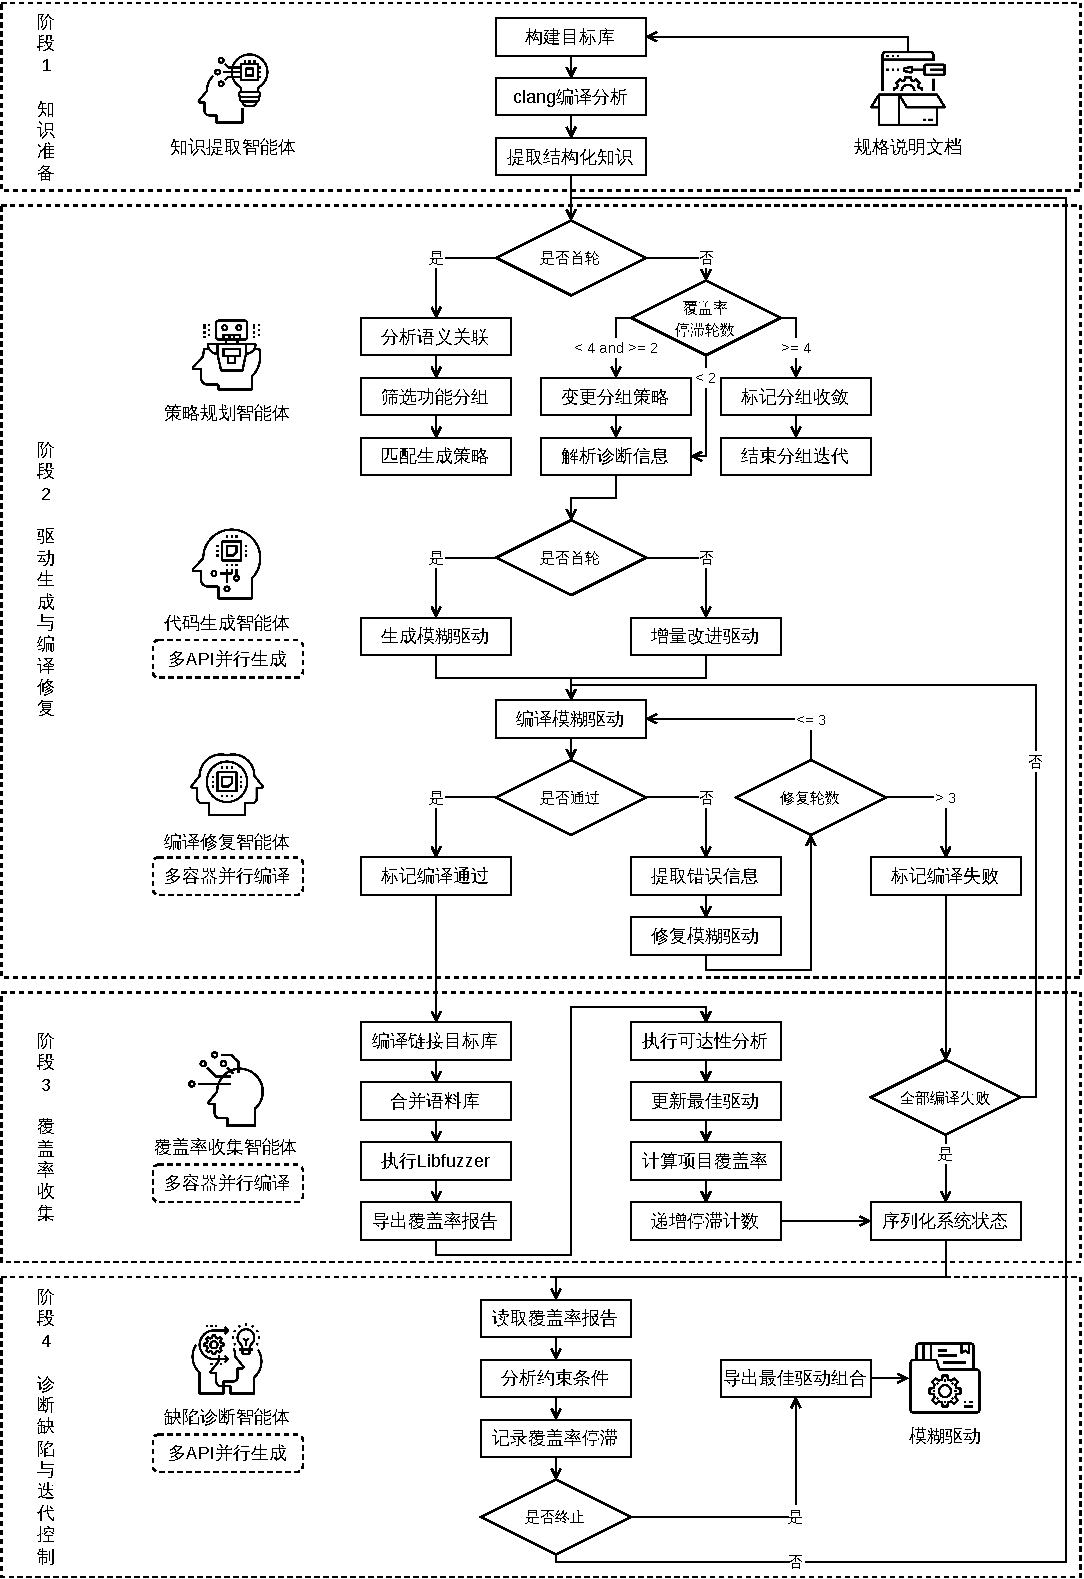
\includegraphics[width=\textwidth]{images/flowchart.drawio.pdf}}
    \caption{MAGIC4FDG系统整体流程图}
    \label{fig:flowchart}
\end{figure}

\textbf{知识准备阶段。}流水线的第一步交给知识提取智能体（Knowledge Agent）完成。该智能体先在Docker容器内编译目标库，随后借助clang前端执行AST导出。导出内容涵盖公开API的函数签名、参数类型与语义标注、函数间调用图，以及宏常量和枚举定义。值得一提的是，首次构建的产物会被缓存到宿主机上，后续轮次只需以只读方式挂载，省去重复编译的开销。整个知识准备仅在流水线启动时执行一次，其产出构成全局知识库，贯穿后续所有迭代轮次。

\textbf{驱动生成与编译修复阶段。}这个阶段涉及三个智能体的协作：策略规划（Planner Agent）、代码生成（Generation Agent）和编译修复（Patching Agent）。

策略规划智能体在知识提取完成后启动工作。首轮迭代属于探索阶段，它加载策略库里十种预定义策略的元数据，每种策略用结构化格式声明适用条件、最佳场景和不兼容约束，同时附带一段策略正文作为提示词后缀。智能体调用LLM分析目标库API之间的语义关系和功能分组，把策略元数据的适用条件跟API特征做匹配，给每个驱动槽位选一个最合适的策略。这里的关键在于，不同槽位会拿到完全不同的策略后缀，从而在代码生成环节产出风格迥异的驱动。如果LLM调用失败，系统回退到基于调用图的规则引擎做确定性匹配。到了后续轮次（利用阶段），策略规划智能体不再调LLM，而是根据各槽位的覆盖率停滞情况决定是否切换策略或标记收敛，同时从缺口诊断结果中提取额外的目标API补充到对应槽位的生成上下文里。

代码生成智能体根据规划结果并行生成驱动代码。它的提示由三部分拼接而成：基础模板（库名、接口规范、通用约束）、API知识上下文（目标API的签名、类型、调用关系）、策略提示词后缀（由Planner匹配的策略正文）。首轮是从零生成，LLM基于这三部分合成完整驱动；后续轮次是增量改进，提示里额外包含当前最佳代码、Analyst输出的结构化约束、以及跨轮次累积的经验知识，要求模型保留已有覆盖路径并定向扩展新路径。

编译修复智能体对所有生成的变体做编译验证和错误修复。每个变体在Docker容器内用带ASan插桩的方式编译，跟目标库静态链接。编译通过则标记成功；未通过的，提取编译器报错，将代码和错误信息注入修复提示模板由LLM修复，最多尝试三次。

编译修复完成后，系统做第一个条件路由判断，只要有至少一个变体编译通过，就进入下一阶段；如果全部失败，则跳过模糊测试直接进入状态持久化，避免无效执行。

\textbf{模糊测试与覆盖率收集阶段。}覆盖率收集智能体（Coverage Agent）负责跑模糊测试并收集精确的覆盖率数据。对每个编译通过的变体，它在Docker容器里依次做这几件事：先用覆盖率插桩标志重新编译驱动并链接目标库；然后合并种子语料库和历史累积语料库，以LibFuzzer的fork模式跑模糊测试。fork模式让每个输入在独立子进程里执行，某个输入触发崩溃不会终止整个测试进程；测试结束后通过语料库重放收集完整覆盖率数据（fork模式下profraw可能写不完整，因此需要重放一遍）；最后用LLVM工具链合并原始数据并导出行级与分支级覆盖率报告。另外，这个智能体还会做控制流图可达性分析，把结构上不可达的代码行标记出来，免得后面Analyst在这些行上浪费精力。覆盖率收集完毕后，系统逐槽位比对本轮与历史最佳覆盖率。若有提升则替换最佳版本，否则将该槽位的停滞计数加一。项目级覆盖率取所有槽位覆盖行的并集。

随后流水线进入状态持久化节点（Checkpoint Node）。这一节点不涉及LLM调用，职责单一，即把当前完整的流水线状态（含各变体源码）序列化为检查点文件写入磁盘。有了这份快照，用户可以从任意已完成的轮次恢复执行。

\textbf{缺口诊断与迭代控制阶段。}这一阶段由Analyst Agent主导。它逐一审视每个活跃槽位的覆盖率缺口，尝试定位根因。具体做法是：读取该槽位当前最佳代码、未覆盖行列表和函数级覆盖率数据，连同API知识上下文一并注入分析提示模板，交由LLM完成诊断。LLM返回的是结构化结果，输出分为三部分：约束列表（要触发某个分支需满足的前置条件）、未覆盖代码簇（按功能分组的未覆盖区域）、以及新发现的知识点。这些内容会追加到该槽位自身的知识空间里，轮次之间持续累积，使系统在迭代中逐步加深对目标库的理解。

Analyst完成分析后，系统做第二个条件路由判断，检查四个终止条件：项目级覆盖率达到用户设定的目标、迭代轮次到上限、所有槽位都已收敛、或者项目级覆盖率连续多轮没有明显提升。满足任何一个就终止迭代，输出各槽位的最佳版本并生成实验报告；否则回到策略规划智能体开始新一轮，进入利用阶段的闭环优化。

\section{需求分析}

MAGIC4FDG的核心功能是为C/C++开源库自动生成高质量模糊驱动，并通过覆盖率反馈迭代持续优化。除此之外，系统还需具备可扩展性、可靠性、可恢复性等非功能性需求。下面从涉众分析出发，明确谁会使用本系统、他们关心什么，再逐一梳理功能性和非功能性需求，最后给出用例图和用例描述。

\subsection{涉众分析}

根据技术背景和使用目的的不同，MAGIC4FDG系统的涉众可以分为三类：目标项目开发者、模糊测试使用者和模糊测试研究人员。表\ref{tab:stakeholder}列出了这三类涉众的特征和期望。

\begin{table}[H]
    \centering
    \caption{涉众分析结果}
    \makebox[\textwidth]{
    \begin{tabular}{ |c|p{5.2cm}|p{5.2cm}| }
        \hline
        \textbf{涉众名称} & \textbf{涉众特征} & \textbf{涉众期望} \\
        \hline
        \textbf{目标项目开发者} &
        被选为测试对象的开源项目的维护者，通常具备较强的C/C++工程能力，熟悉自身接口设计与使用语义，了解模糊测试平台的基本要求。该类涉众直接参与项目构建与接口演进，对系统产出的驱动可用性与行为一致性有要求。 &
        希望系统能够在不破坏接口契约的前提下，自动生成结构完整、逻辑合理、覆盖真实调用路径的模糊测试驱动，用于集成测试、安全审计或接口验证，降低人工编写负担并提高测试质量。 \\
        \hline
        \textbf{模糊测试使用者} &
        使用LibFuzzer、AFL或OSS-Fuzz等平台执行模糊测试的测试工程师或安全研究人员，关注模糊驱动的适配性与执行效果。该类涉众具备模糊测试实践经验，熟悉驱动编写规范与覆盖率评估方法，但不一定深入了解目标库的内部实现。 &
        希望系统生成的驱动能够直接用于主流模糊测试引擎，具备较高的代码覆盖率和缺陷发现能力；同时期望系统提供覆盖率报告和迭代过程记录，便于评估测试效果和定位潜在漏洞。 \\
        \hline
        \textbf{模糊测试研究人员} &
        从事模糊测试自动化、驱动生成或大语言模型辅助测试等方向研究的学者或研究工程师。该类涉众关注系统的技术方法与创新点，通常将本系统与其他工具进行对比实验以验证方法的有效性。 &
        希望系统具备良好的可复现性和可配置性，能够在不同目标库上稳定运行；同时期望系统提供详细的实验数据（覆盖率变化曲线、迭代轮次统计、消融实验支持等），便于进行公平的横向对比和方法分析。 \\
        \hline
    \end{tabular}}
    \label{tab:stakeholder}
\end{table}

三类涉众的差异主要体现在技术背景和关注重点上。目标项目开发者关注驱动是否符合API使用规范及缺陷发现能力；模糊测试使用者关注覆盖率、崩溃数量及与现有测试基础设施的兼容性；模糊测试研究人员则更关注实验数据和配置灵活性。三者共同期望系统能够在减少人工干预的同时保证驱动质量。

\subsection{功能性需求分析}

在调研现有工具的基础上，本文梳理出七个方面的功能性需求：目标库配置与知识提取、策略规划与驱动生成、编译修复、模糊测试与覆盖率收集、缺口诊断与迭代优化、状态持久化与恢复、实验报告生成。具体内容见表\ref{tab:functional-req}。

\begin{table}[H]
    \centering
    \caption{功能性需求列表}
    \label{tab:functional-req}
    \makebox[\textwidth]{
    \begin{tabular}{ |c|p{3.8cm}|p{8cm}| }
        \hline
        \textbf{需求编号} & \textbf{需求名称} & \textbf{需求描述} \\
        \hline
        \textbf{R1} & 目标库配置与知识提取 & 用户可以通过配置文件指定目标C/C++库的构建方式、头文件路径和静态库路径，系统自动在Docker容器内完成构建并提取API知识 \\
        \hline
        \textbf{R2} & 策略规划与驱动生成 & 系统应能够根据目标库的API特征自动匹配合适的模糊策略，并基于策略指导生成多个风格互补的模糊驱动代码 \\
        \hline
        \textbf{R3} & 编译修复 & 系统应能够对生成的驱动代码执行编译验证，对编译失败的变体自动诊断错误原因并尝试修复 \\
        \hline
        \textbf{R4} & 模糊测试执行 & 系统应能够对编译成功的驱动在隔离环境中执行模糊测试，支持崩溃隔离和语料库累积 \\
        \hline
        \textbf{R5} & 覆盖率收集与分析 & 系统应能够收集行级与分支级覆盖率数据，执行可达性分析过滤不可达代码，并维护每个驱动的最佳版本记录 \\
        \hline
        \textbf{R6} & 缺口诊断与迭代优化 & 系统应能够对覆盖率缺口进行根因分析，输出结构化约束描述，并基于分析结果在后续轮次中定向改进驱动代码 \\
        \hline
        \textbf{R7} & 状态持久化与恢复 & 系统应能够在每轮迭代后保存完整的流水线状态，支持从任意检查点恢复执行 \\
        \hline
        \textbf{R8} & 实验报告生成 & 系统应能够在迭代结束后生成包含覆盖率统计、迭代历史和最佳驱动代码的实验报告 \\
        \hline
    \end{tabular}}
\end{table}

目标库配置与知识提取（R1）是一切的起点。用户编写一个JSON配置文件，将库名、构建命令、头文件路径、静态库路径等信息填入即可。系统拿到配置后在Docker里编译目标库，然后用clang AST导出拿到结构化的API知识，包括函数签名、参数类型、调用图、宏常量等。这步的产出是一个全局知识库，后续所有智能体都从这里获取信息。

策略规划与驱动生成（R2）是整个系统最核心的部分。规划环节分析API的特征和适合的测试策略，然后给每个槽位分配一个；生成环节拿着分配好的策略后缀、API知识和基础模板去调LLM，让它写出完整的模糊驱动代码。第一轮从零开始写，后续轮次则在已有代码上做增量改进。

编译修复（R3）的目的很直接——保证代码能编译通过。变体逐个送入Docker容器，以带ASan插桩的方式编译并与目标库静态链接。编译未通过时，系统提取编译器报错交给LLM尝试修复，上限三次，超过即放弃。之所以设定三次而非更多，是在修复成本与收益之间做的权衡——实践中绝大多数可修复的错误在前两轮就能解决，第三轮仍失败的往往涉及设计层面的问题。保住尽可能多的变体，后续模糊测试才有足够的样本量。

模糊测试执行（R4）与覆盖率收集与分析（R5）共同构成测试与反馈环节。前者在Docker容器内以fork模式运行LibFuzzer，每个输入在独立子进程中执行，单个崩溃不会拖垮整体测试进程。后者负责精确度量，通过语料库重放（非fork模式）配合LLVM工具链，导出行级与分支级覆盖率数据。此外，系统还执行控制流图可达性分析，将结构上不可达的代码行预先标记，避免后续诊断环节在这些行上做无用功。

缺口诊断与迭代优化（R6）是覆盖率能够持续攀升的关键所在。Analyst针对每个槽位的未覆盖代码做根因分析，产出两类结构化信息：约束列表（触发特定分支所需的前置条件）和未覆盖代码簇（按功能聚类的未覆盖区域）。这些信息被写入各槽位独立的知识空间，轮次间不断累积。到了后续迭代，Generation Agent读取这些约束作为增量改进的精确指引，相当于把"哪里没覆盖、为什么没覆盖"的诊断结论直接转化为生成指令。

状态持久化与恢复（R7）保障容错能力。每轮迭代完成后，系统把完整的流水线状态序列化为检查点文件，包括所有槽位的最佳代码、覆盖率数据、累积知识和迭代计数。异常中断时用户可以指定检查点恢复执行，无需从头开始。

实验报告生成（R8）满足用户对结果的查阅需求。迭代终止后系统自动生成包含项目级覆盖率统计、各槽位覆盖率对比、迭代历史和最佳驱动源码的结构化报告，方便评估效果和做横向对比。

\subsection{非功能性需求分析}

功能性需求之外，非功能性需求同样重要。本文将其分为质量属性、性能需求和约束三部分，具体见表\ref{tab:nonfunctional-req}。

\begin{table}[H]
    \centering
    \caption{非功能性需求列表}
    \label{tab:nonfunctional-req}
    \makebox[\textwidth]{
    \begin{tabular}{ |c|c|p{3cm}|p{7cm}| }
        \hline
        \textbf{需求编号} & \textbf{需求类型} & \textbf{需求名称} & \textbf{需求描述} \\
        \hline
        \textbf{QA1} & 质量属性 & 可扩展性 & 系统应支持通过配置文件接入新的目标库，无需修改系统源码 \\
        \hline
        \textbf{QA2} & 质量属性 & 可靠性 & 系统生成的驱动在经过编译修复后应达到60\%以上的编译通过率 \\
        \hline
        \textbf{QA3} & 质量属性 & 可恢复性 & 系统应支持从任意轮次的检查点恢复执行，恢复后状态与中断前一致 \\
        \hline
        \textbf{QA4} & 质量属性 & 隔离性 & 所有编译、模糊测试和覆盖率收集操作应在Docker容器内执行，不影响宿主机环境 \\
        \hline
        \textbf{QA5} & 质量属性 & 可复现性 & 在相同配置和相同大语言模型下，系统的覆盖率结果应具备统计意义上的可复现性 \\
        \hline
        \textbf{PR1} & 性能需求 & 并行处理能力 & 系统应支持多个驱动变体的并行生成、并行编译和并行模糊测试 \\
        \hline
        \textbf{PR2} & 性能需求 & 构建缓存 & 目标库首次构建后应缓存产物，后续轮次的编译和模糊测试应复用缓存，避免重复构建 \\
        \hline
        \textbf{CS1} & 约束 & 开发语言 & 系统使用Python语言进行开发 \\
        \hline
        \textbf{CS2} & 约束 & 容器化依赖 & 系统运行依赖Docker引擎和LLVM工具链 \\
        \hline
    \end{tabular}}
\end{table}

质量属性方面本文列出五条，其中最重要的两条是可扩展性（QA1）和隔离性（QA4）。可扩展性的含义是，用户更换目标库时只需修改配置文件，系统代码本身不动。这一点直接决定了系统能否脱离实验室环境、真正被他人使用。隔离性则依赖Docker容器化来兑现，构建、模糊测试均在容器内完成，宿主机环境不受影响，多个库并行运行时也彼此隔离。可靠性（QA2）要求编译修复环节切实有效，每轮需保证足够数量的变体编译通过，否则后续测试无从谈起。可恢复性（QA3）通过检查点机制实现，中断后从最近的检查点恢复即可继续。可复现性（QA5）是实验评估的基本前提，本文通过固定随机种子与确定性调度两项措施加以保障。

性能需求方面，系统需要在代码生成、编译修复和模糊测试三个环节支持多变体并行执行（PR1）。这三个环节的计算相互独立，并行化能显著缩短单轮迭代耗时，充分利用多核资源。构建缓存（PR2）则要求目标库的编译产物在首次构建后持久化存储，后续轮次一律通过只读挂载复用，杜绝每轮重复构建带来的时间浪费。

约束方面，系统用Python开发（CS1），利用其丰富的生态支持LLM调用和流水线编排；运行依赖Docker引擎提供容器化执行环境，依赖LLVM工具链提供覆盖率插桩和数据导出能力（CS2）。

\subsection{系统用例图}

基于前面的涉众分析和功能性需求，本文对相关描述进行了实体识别、用例拆分和筛选，构建了系统用例图，如图\ref{fig:usecase}所示。

系统包含10个用例：配置目标库、提取API知识、规划模糊策略、生成模糊驱动、修复编译错误、执行模糊测试、收集覆盖率数据、诊断覆盖率缺口、恢复中断任务、查看实验报告。参与者有五类：三类人类参与者（目标项目开发者、模糊测试使用者、模糊测试研究人员）和两类外部系统参与者（Docker引擎、大语言模型服务）。

三类人类参与者都可以使用配置目标库、恢复中断任务和查看实验报告。提取API知识、规划模糊策略、生成模糊驱动、修复编译错误、执行模糊测试、收集覆盖率数据和诊断覆盖率缺口这七个用例是系统内部自动执行的流程，用户启动任务后由系统自动编排。Docker引擎参与知识提取、编译修复、模糊测试和覆盖率收集四个用例；大语言模型服务参与策略规划、驱动生成、编译修复和缺口诊断四个用例。

\begin{figure}[H]
    \centering
    \makebox[\textwidth]{
    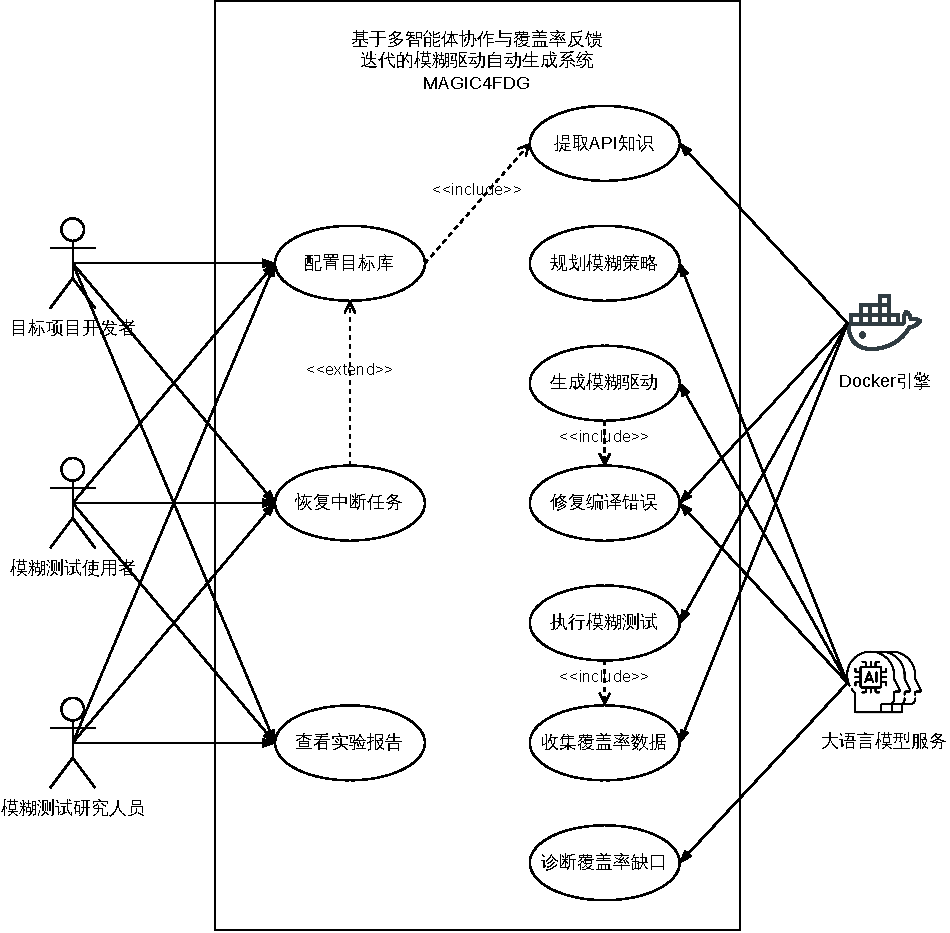
\includegraphics[width=\textwidth]{images/usecase.drawio.pdf}}
    \caption{MAGIC4FDG系统用例图}
    \label{fig:usecase}
\end{figure}

\subsection{系统用例描述}

上面的用例图从用户视角展示了系统行为与需求之间的关系。下面逐一描述每个用例的细节，帮助理解系统功能并指导后续设计。

配置目标库是用户使用系统的入口。用户编写JSON配置文件声明目标库的构建方式和路径信息，通过命令行参数控制迭代轮次、目标覆盖率等运行时行为，系统据此启动自动化流程。表\ref{tab:uc1}是该用例的详细描述。

\begin{table}[H]
    \centering
    \caption{用例"配置目标库"详细描述}
    \label{tab:uc1}
    \makebox[\textwidth]{
    \begin{tabular}{ |c|p{12cm}| }
        \hline
        \textbf{用例编号} & UC1 \\
        \hline
        \textbf{用例名称} & 配置目标库 \\
        \hline
        \textbf{参与者} & 目标项目开发者、模糊测试使用者、模糊测试研究人员 \\
        \hline
        \textbf{前置条件} & 目标库源码可通过网络获取，用户了解目标库的构建方式 \\
        \hline
        \textbf{后置条件} & 系统获得有效的目标库配置，可启动自动化生成流程 \\
        \hline
        \textbf{基本流程} &
        1. 用户编写目标库配置文件，指定库名、构建命令、头文件路径、静态库路径和覆盖率源文件路径 \newline
        2. 用户通过命令行指定配置文件路径和运行参数（最大轮次、目标覆盖率、模糊测试时长等） \newline
        3. 系统验证配置文件格式和必填字段的完整性 \newline
        4. 系统启动流水线执行 \\
        \hline
        \textbf{扩展流程} & 3a. 配置文件格式错误或缺少必填字段时，系统输出错误提示并终止 \\
        \hline
    \end{tabular}}
\end{table}

提取API知识是获取目标库结构化信息的基础操作。系统利用clang前端的AST导出能力，在Docker容器内精确提取函数签名、参数类型、调用图和宏常量定义，构建产物缓存到宿主机避免后续重复构建。表\ref{tab:uc2}是该用例的详细描述。

\begin{table}[H]
    \centering
    \caption{用例"提取API知识"详细描述}
    \label{tab:uc2}
    \begin{tabular}{ |c|p{12cm}| }
        \hline
        \textbf{用例编号} & UC2 \\
        \hline
        \textbf{用例名称} & 提取API知识 \\
        \hline
        \textbf{参与者} & Docker引擎 \\
        \hline
        \textbf{前置条件} & 系统获得有效的目标库配置 \\
        \hline
        \textbf{后置条件} & 系统获得目标库的结构化API知识（函数签名、调用图、类型信息） \\
        \hline
        \textbf{基本流程} &
        1. 系统在Docker容器内执行目标库的构建命令 \newline
        2. 系统通过clang AST导出提取头文件和源文件中的API信息 \newline
        3. 系统解析AST JSON，提取函数签名、参数类型、调用图和宏定义 \newline
        4. 系统将构建产物缓存至宿主机 \newline
        5. 系统将提取结果存入全局知识库 \\
        \hline
        \textbf{扩展流程} & 1a. 构建失败时，系统输出构建日志并终止流程 \\
        \hline
    \end{tabular}
\end{table}

规划模糊策略是为每个槽位选择最合适生成策略的决策环节。探索阶段，Planner通过LLM把策略库中十种策略与目标库API特征做匹配；利用阶段，根据覆盖率停滞情况动态调整策略分配。表\ref{tab:uc3}是该用例的详细描述。

\begin{table}[H]
    \centering
    \caption{用例"规划模糊策略"详细描述}
    \label{tab:uc3}
    \begin{tabular}{ |c|p{12cm}| }
        \hline
        \textbf{用例编号} & UC3 \\
        \hline
        \textbf{用例名称} & 规划模糊策略 \\
        \hline
        \textbf{参与者} & 大语言模型服务 \\
        \hline
        \textbf{前置条件} & 系统已完成API知识提取 \\
        \hline
        \textbf{后置条件} & 每个模糊驱动获得匹配的生成策略和目标API列表 \\
        \hline
        \textbf{基本流程} &
        1. 系统加载策略库中十种模糊策略的元数据 \newline
        2. 系统将API知识注入规划提示模板 \newline
        3. 系统调用大语言模型分析API语义关系并匹配策略 \newline
        4. 系统为每个模糊驱动分配目标API和对应策略 \\
        \hline
        \textbf{扩展流程} & 3a. 大语言模型调用失败时，系统回退至基于调用图的规则引擎进行确定性匹配 \\
        \hline
    \end{tabular}
\end{table}

生成模糊驱动是核心的代码生成环节。每个槽位接收差异化的策略后缀，引导LLM采用不同的代码结构和API调用模式；首轮从零生成，后续轮次切换为基于约束和累积经验的增量改进。表\ref{tab:uc4}是该用例的详细描述。

\begin{table}[H]
    \centering
    \caption{用例"生成模糊驱动"详细描述}
    \label{tab:uc4}
    \begin{tabular}{ |c|p{12cm}| }
        \hline
        \textbf{用例编号} & UC4 \\
        \hline
        \textbf{用例名称} & 生成模糊驱动 \\
        \hline
        \textbf{参与者} & 大语言模型服务 \\
        \hline
        \textbf{前置条件} & 策略规划完成，每个驱动已分配目标API和策略 \\
        \hline
        \textbf{后置条件} & 系统获得多个模糊驱动代码变体 \\
        \hline
        \textbf{基本流程} &
        1. 系统为每个驱动组装提示（基础模板+API知识+策略后缀） \newline
        2. 系统并行调用大语言模型生成驱动代码 \newline
        3. 系统从模型输出中提取代码块并保存为变体文件 \\
        \hline
        \textbf{扩展流程} & 2a. 后续轮次，提示额外包含最佳代码、约束列表和累积经验 \\
        \hline
    \end{tabular}
\end{table}

修复编译错误保证生成的代码能通过编译。编译修复智能体在Docker容器内做带ASan插桩的编译，失败的变体提取错误信息让LLM修复，最多三次。表\ref{tab:uc5}是该用例的详细描述。

\begin{table}[H]
    \centering
    \caption{用例"修复编译错误"详细描述}
    \label{tab:uc5}
    \begin{tabular}{ |c|p{12cm}| }
        \hline
        \textbf{用例编号} & UC5 \\
        \hline
        \textbf{用例名称} & 修复编译错误 \\
        \hline
        \textbf{参与者} & Docker引擎、大语言模型服务 \\
        \hline
        \textbf{前置条件} & 代码生成智能体已输出驱动变体 \\
        \hline
        \textbf{后置条件} & 变体被标记为编译成功或编译失败（已耗尽重试次数） \\
        \hline
        \textbf{基本流程} &
        1. 系统在Docker容器内对变体执行带插桩的编译 \newline
        2. 编译成功，标记变体为通过 \\
        \hline
        \textbf{扩展流程} &
        1a. 编译失败时，系统提取错误信息并调用大语言模型生成修复代码 \newline
        1b. 重新编译修复后的代码，最多重试三次 \newline
        1c. 三次重试均失败，标记变体为编译失败 \\
        \hline
    \end{tabular}
\end{table}

执行模糊测试是对目标库做自动化安全测试的核心环节。fork模式让每个输入在独立子进程里跑，单个崩溃不会终止整个测试；每轮发现的有效输入持久化存储供后续轮次复用。表\ref{tab:uc6}是该用例的详细描述。

\begin{table}[H]
    \centering
    \caption{用例"执行模糊测试"详细描述}
    \label{tab:uc6}
    \begin{tabular}{ |c|p{12cm}| }
        \hline
        \textbf{用例编号} & UC6 \\
        \hline
        \textbf{用例名称} & 执行模糊测试 \\
        \hline
        \textbf{参与者} & Docker引擎 \\
        \hline
        \textbf{前置条件} & 存在至少一个编译成功的驱动变体 \\
        \hline
        \textbf{后置条件} & 系统获得模糊测试产生的语料库和崩溃样本 \\
        \hline
        \textbf{基本流程} &
        1. 系统以覆盖率插桩标志重新编译驱动变体 \newline
        2. 系统合并种子语料库与历史累积语料库 \newline
        3. 系统以fork模式运行LibFuzzer执行模糊测试 \newline
        4. 系统收集测试产生的新语料库和崩溃样本 \\
        \hline
        \textbf{扩展流程} & 3a. 所有变体均编译失败时，跳过本用例直接进入状态持久化 \\
        \hline
    \end{tabular}
\end{table}

收集覆盖率数据是获取精确反馈的关键环节。fork模式下profraw文件可能写不完整，所以系统通过语料库重放在非fork模式下重新执行所有输入来保证数据完整性，同时维护每个槽位的最佳版本记录和停滞计数。表\ref{tab:uc7}是该用例的详细描述。

\begin{table}[H]
    \centering
    \caption{用例"收集覆盖率数据"详细描述}
    \label{tab:uc7}
    \begin{tabular}{ |c|p{12cm}| }
        \hline
        \textbf{用例编号} & UC7 \\
        \hline
        \textbf{用例名称} & 收集覆盖率数据 \\
        \hline
        \textbf{参与者} & Docker引擎 \\
        \hline
        \textbf{前置条件} & 模糊测试执行完成，语料库已生成 \\
        \hline
        \textbf{后置条件} & 系统获得行级与分支级覆盖率报告，最佳版本记录已更新 \\
        \hline
        \textbf{基本流程} &
        1. 系统通过语料库重放机制收集完整的覆盖率原始数据 \newline
        2. 系统通过LLVM工具链合并数据并导出覆盖率报告 \newline
        3. 系统执行控制流图可达性分析，标记不可达代码行 \newline
        4. 系统比较当前覆盖率与历史最佳，更新最佳版本记录 \newline
        5. 系统计算项目级覆盖率并更新停滞计数 \\
        \hline
        \textbf{扩展流程} & 4a. 当前覆盖率未超过历史最佳时，递增该驱动的停滞计数 \\
        \hline
    \end{tabular}
\end{table}

诊断覆盖率缺口是实现精准迭代改进的智能分析环节。Analyst只输出结构化的约束描述和未覆盖代码簇分析，把"诊断"和"生成"的职责分开；诊断结果持久化到每个槽位的隔离知识空间，跨轮次累积形成经验库。表\ref{tab:uc8}是该用例的详细描述。

\begin{table}[H]
    \centering
    \caption{用例"诊断覆盖率缺口"详细描述}
    \label{tab:uc8}
    \begin{tabular}{ |c|p{12cm}| }
        \hline
        \textbf{用例编号} & UC8 \\
        \hline
        \textbf{用例名称} & 诊断覆盖率缺口 \\
        \hline
        \textbf{参与者} & 大语言模型服务 \\
        \hline
        \textbf{前置条件} & 覆盖率数据收集完成 \\
        \hline
        \textbf{后置条件} & 每个活跃驱动获得结构化的约束列表和未覆盖代码簇分析 \\
        \hline
        \textbf{基本流程} &
        1. 系统读取每个驱动的最佳代码和未覆盖代码行列表 \newline
        2. 系统将覆盖率数据与API知识注入分析提示模板 \newline
        3. 系统调用大语言模型进行根因分析 \newline
        4. 系统将输出的约束和知识追加到驱动的隔离知识空间 \\
        \hline
        \textbf{扩展流程} & 3a. 大语言模型输出格式异常时，系统跳过该驱动的本轮分析 \\
        \hline
    \end{tabular}
\end{table}

恢复中断任务让用户能从之前保存的检查点继续执行。MAGIC4FDG的单次完整运行可能持续数小时（取决于目标库复杂度、迭代轮次和模糊测试时长），期间可能因网络波动、LLM服务不可用或系统资源不足而中断。检查点恢复机制确保用户无需从头开始，可以从最近一次成功完成的轮次继续。表\ref{tab:uc9}是该用例的详细描述。

\begin{table}[H]
    \centering
    \caption{用例"恢复中断任务"详细描述}
    \label{tab:uc9}
    \begin{tabular}{ |c|p{12cm}| }
        \hline
        \textbf{用例编号} & UC9 \\
        \hline
        \textbf{用例名称} & 恢复中断任务 \\
        \hline
        \textbf{参与者} & 目标项目开发者、模糊测试使用者、模糊测试研究人员 \\
        \hline
        \textbf{前置条件} & 系统存在之前保存的检查点文件 \\
        \hline
        \textbf{后置条件} & 系统从指定检查点恢复完整的流水线状态并继续迭代 \\
        \hline
        \textbf{基本流程} &
        1. 用户通过命令行参数指定检查点文件路径 \newline
        2. 系统反序列化检查点文件，恢复流水线状态 \newline
        3. 系统从恢复的轮次继续执行迭代流程 \\
        \hline
        \textbf{扩展流程} & 2a. 检查点文件损坏或格式不兼容时，系统输出报错并终止 \\
        \hline
    \end{tabular}
\end{table}

查看实验报告让用户了解系统的运行结果和测试效果。对三类涉众来说，报告是评估系统产出质量的主要途径——开发者通过它了解驱动覆盖了哪些API路径、发现了哪些缺陷；测试使用者通过它评估覆盖率水平和崩溃发现能力；研究人员通过其中的定量数据做横向对比。报告同时以Markdown和JSON两种格式输出，兼顾可读性和自动化处理需求。表\ref{tab:uc10}是该用例的详细描述。 

\begin{table}[H]
    \centering
    \caption{用例"查看实验报告"详细描述}
    \label{tab:uc10}
    \begin{tabular}{ |c|p{12cm}| }
        \hline
        \textbf{用例编号} & UC10 \\
        \hline
        \textbf{用例名称} & 查看实验报告 \\
        \hline
        \textbf{参与者} & 目标项目开发者、模糊测试使用者、模糊测试研究人员 \\
        \hline
        \textbf{前置条件} & 系统迭代终止（满足任一终止条件） \\
        \hline
        \textbf{后置条件} & 用户获得包含覆盖率统计和最佳驱动代码的结构化报告 \\
        \hline
        \textbf{基本流程} &
        1. 系统在迭代终止后自动生成Markdown和JSON格式的实验报告 \newline
        2. 报告包含项目级覆盖率、各驱动覆盖率对比、迭代历史和最佳驱动源码 \newline
        3. 用户查阅报告评估测试效果 \\
        \hline
        \textbf{扩展流程} & 1a. 用户可通过配置选择报告中包含的内容项 \\
        \hline
    \end{tabular}
\end{table}

\section{系统概要设计}

本节用"4+1"视图方法描述MAGIC4FDG的架构。"4+1"视图包含逻辑视图、开发视图、进程视图、物理视图和场景视图五部分，其中场景视图就是3.2节的用例视图，已经在需求分析阶段完成了。下面先介绍整体架构设计，再从模块划分、逻辑视图、开发视图、进程视图和物理视图四个维度展开。

\subsection{系统整体架构设计}

图\ref{fig:architecture}展示了MAGIC4FDG的整体架构。用户提供目标库配置后，系统在Docker容器内依次完成知识提取、驱动生成、编译修复、模糊测试与覆盖率收集、缺口诊断等环节。各环节的产出经由共享状态对象流转，形成迭代反馈闭环以持续优化覆盖率。图中按模块划分了系统功能，箭头标明模块间的依赖方向。

\begin{figure}[htbp]
    \centering
    \makebox[\textwidth]{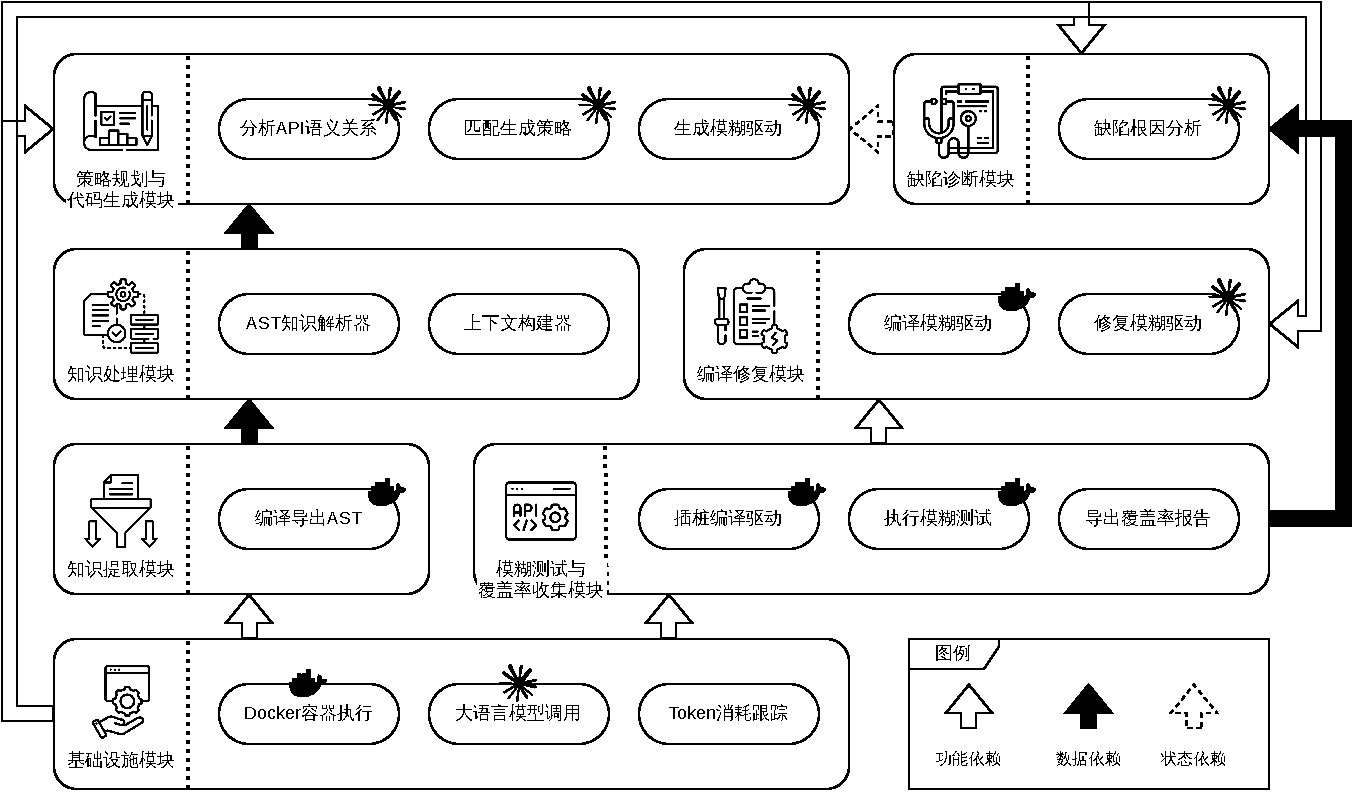
\includegraphics[width=1.1\textwidth]{images/architecture.drawio.pdf}}
    \caption{MAGIC4FDG系统整体架构图}
    \label{fig:architecture}
\end{figure}

架构自底向上分层，共包含七个功能模块，具体包括：基础设施、知识处理、知识提取、策略规划与代码生成、编译修复、模糊测试与覆盖率收集、缺口诊断。

基础设施模块是底座，提供Docker执行、LLM调用和令牌追踪三项服务，其他模块都依赖它。知识处理模块解析clang AST输出，将原始的语法树信息转换为各智能体能直接使用的文本片段。知识提取模块在Docker里编译目标库、做AST导出，产出全局知识库。策略规划与代码生成模块是核心，负责分析API语义、匹配策略、并行生成多个风格不同的驱动。编译修复模块负责将编译失败的变体修复。模糊测试与覆盖率收集模块执行测试、收集数据。缺口诊断模块分析哪里没覆盖到、为什么没覆盖到，输出约束供下一轮使用。各模块的详细设计在下一小节展开。

\subsection{系统模块划分}

在需求分析的基础上做模块化划分，可以有效降低系统复杂度，让结构更清晰。MAGIC4FDG按功能职责分为七个模块，下面逐一介绍，最后解释模块间的依赖关系。

\textbf{基础设施模块。}该模块并不直接对应某个功能性需求或用例，但它是其他所有模块赖以运行的技术底座。内部包含三个核心组件。其一，Docker执行器，封装知识提取、编译、模糊测试、覆盖率收集四类容器化操作的命令构建与执行逻辑，同时负责构建缓存的创建与挂载管理，对应QA4（隔离性）和PR2（构建缓存）两项非功能性需求。其二，LLM工厂，以统一接口创建带重试机制的模型客户端实例，集中管理配置参数、超时策略和错误处理。其三，令牌追踪器，按智能体类型分类记录每次模型调用的令牌消耗，供成本监控和实验分析使用。

\textbf{知识处理模块。}对应R1中的知识组织部分。三个组件各负责一项工作：提取器负责解析clang AST的JSON输出，从中提取函数签名、参数类型、调用图和宏常量；上下文构建器根据"谁要用"来决定"给什么"——代码生成智能体需要看目标API的完整签名和调用关系，Analyst需要看未覆盖代码行的上下文，同一份知识给不同智能体的视图是不一样的；分组引擎做基于调用图的API分组和规则引擎策略匹配，当LLM策略规划失败时作为确定性回退。

\textbf{知识提取模块。}对应R1和UC2。功能较为明确，即在Docker容器内编译目标库，用clang前端做AST导出，结果交给知识处理模块去解析。构建产物会缓存到宿主机，后续的编译和模糊测试容器只读挂载即可，无需每轮重新构建。该模块仅执行一次。

\textbf{策略规划与代码生成模块。}对应R2、UC3和UC4，是整个系统的核心。探索阶段加载十种策略的元数据，让LLM分析API之间的语义关系，给每个槽位匹配策略；然后用差异化的提示词并行生成多个驱动。利用阶段则根据覆盖率停滞情况动态调整策略，将Analyst的约束和历史经验注入提示词做增量改进。

\textbf{编译修复模块。}对应R3和UC5。对每个变体在Docker容器内做带ASan插桩的编译和静态链接。编译通过则标记成功；未通过的提取错误信息由LLM修复，最多三次。该模块的存在让系统对LLM代码生成质量有容错能力，保证每轮有足够变体进入模糊测试。

\textbf{模糊测试与覆盖率收集模块。}对应R4、R5、UC6和UC7。对每个编译通过的变体，在Docker容器内依次做：覆盖率插桩重编译、合并语料库、fork模式模糊测试、语料库重放收集完整覆盖率、LLVM工具链导出行级与分支级报告。还做控制流图可达性分析过滤不可达代码行，并维护各槽位的最佳版本记录和停滞计数。

\textbf{缺口诊断模块。}对应R6和UC8。对每个活跃槽位，读取最佳代码和未覆盖代码行列表，把覆盖率数据与API知识注入分析提示模板让LLM做根因分析。输出结构化的约束列表和未覆盖代码簇，追加到对应槽位的隔离知识空间，跨轮次累积，为后续的策略规划与代码生成提供精确的改进指导。

\textbf{模块之间的依赖关系。}图\ref{fig:architecture}的架构是基于需求分析得到的功能性需求和用例做模块化划分的结果，模块间存在数据依赖、功能依赖和状态依赖三类关系。整体上看，系统采用分层架构，上层依赖下层，下层不依赖上层，符合依赖倒置原则，有效降低了耦合度。

具体来说：知识提取模块对基础设施模块是功能依赖（调用Docker执行器在容器内完成构建和AST导出），对知识处理模块是数据依赖（调用提取器解析AST JSON并构建知识库）。策略规划与代码生成模块、缺口诊断模块对知识处理模块是数据依赖，它们需要知识处理模块提供的结构化API知识和格式化上下文文本。所有涉及LLM调用的模块对基础设施模块是功能依赖，基础设施模块提供LLM调用服务和Docker执行服务。编译修复模块和模糊测试与覆盖率收集模块对基础设施模块同样是功能依赖，都通过Docker执行器在容器内完成各自的工作。缺口诊断模块与策略规划与代码生成模块之间是状态依赖，Analyst的输出（约束列表和累积知识）通过共享的流水线状态对象传递给后者，后者在后续轮次中据此调整生成策略和提示词内容。

\subsection{系统逻辑视图}

逻辑视图关注功能性需求，描述系统的主要组件、类和它们之间的关系，通常用类图表示。图\ref{fig:logic-view}是MAGIC4FDG的逻辑视图。

\begin{figure}[htbp]
    \centering
    \makebox[\textwidth]{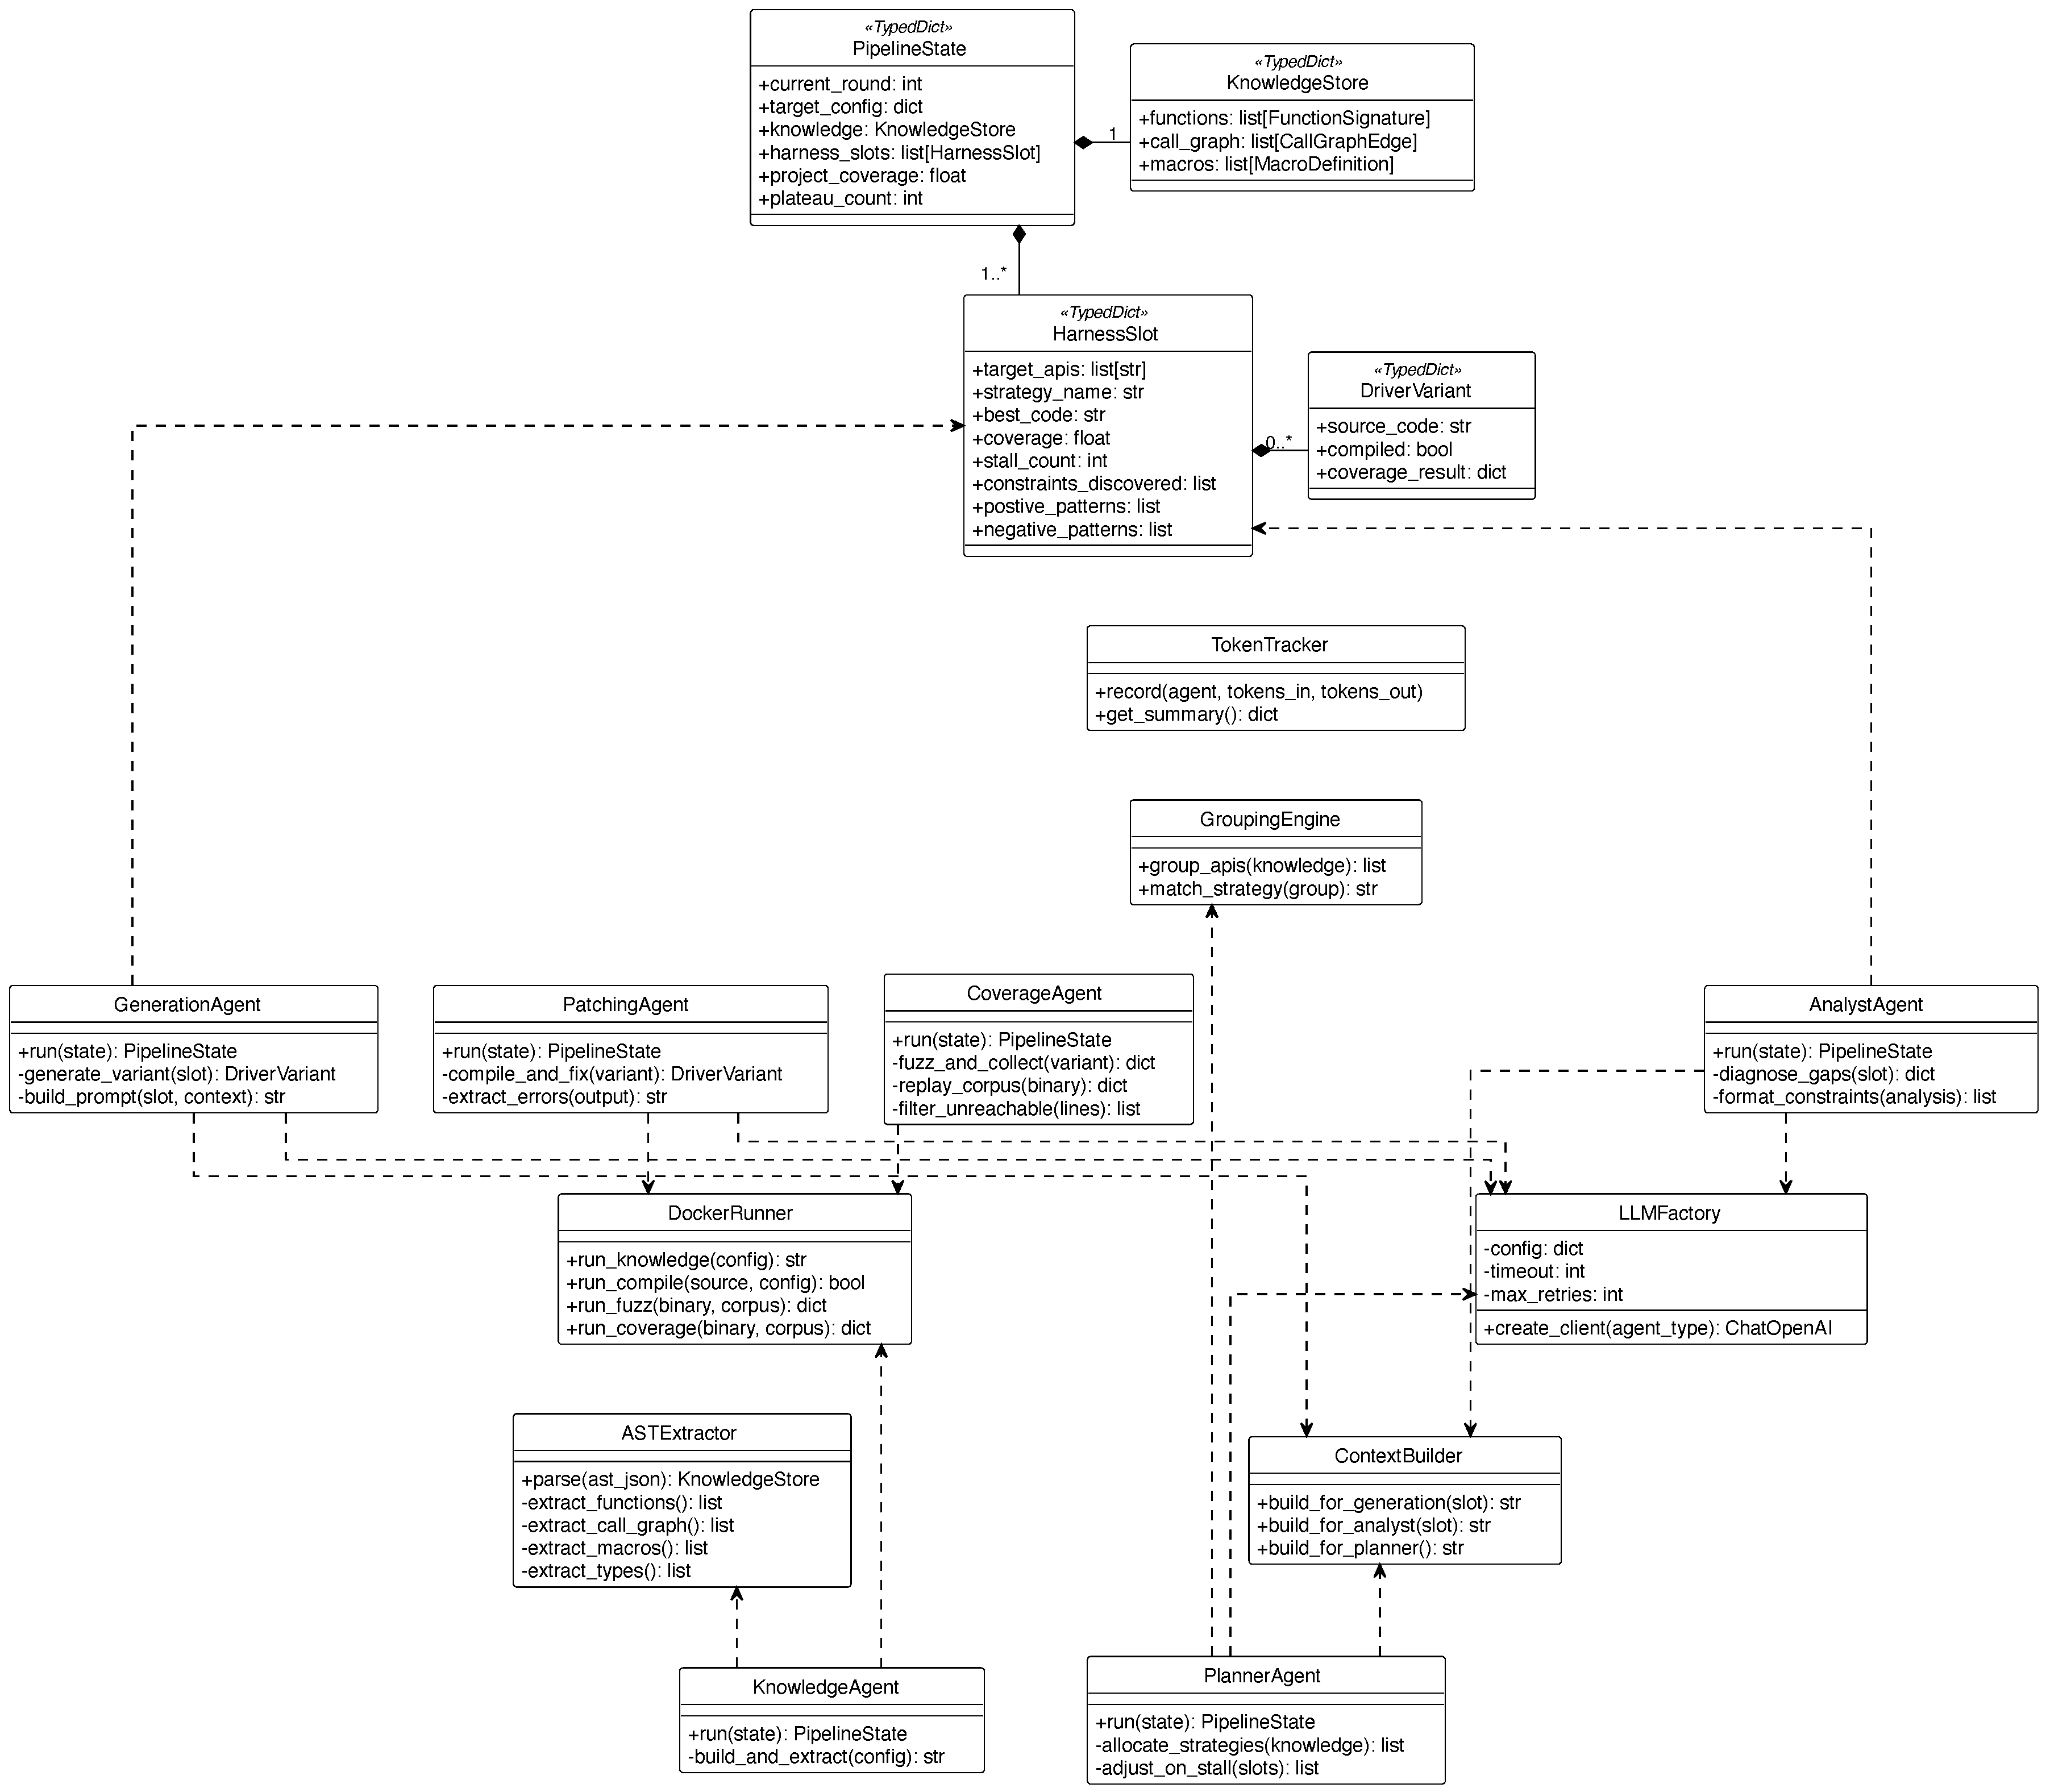
\includegraphics[width=1.2\textwidth]{images/logic_view.pdf}}
    \caption{MAGIC4FDG系统逻辑视图}
    \label{fig:logic-view}
\end{figure}

这个逻辑视图用概念类图展示系统的静态结构。在看各模块的类之前，先说明全局状态，这是理解整个系统数据流的关键。MAGIC4FDG用共享状态架构，模块之间靠一个统一的状态对象传数据。这个状态由四个类型支撑：PipelineState是最外层的容器，TypedDict定义，包含当前轮次、目标库配置、知识库、槽位列表等信息，所有模块都通过它交换信息；HarnessSlot代表一个独立的驱动槽位，里面有目标API列表、策略名、最佳代码、覆盖率、停滞计数和累积知识，这是整个系统中最核心的数据结构，因为多驱动并行迭代全靠它；DriverVariant相对简单，表示单轮生成的一个变体，包含源码、编译状态和覆盖率；KnowledgeStore存储全局知识，包括函数签名、调用图、宏定义等。

下面按3.3.2的模块划分，分别介绍各模块的核心类。

\textbf{基础设施模块}包含DockerRunner、LLMFactory和TokenTracker三个类。DockerRunner封装四类Docker操作（知识提取、编译、模糊测试、覆盖率收集），每类对应一个方法，内部负责命令构建、卷挂载管理和容器输出解析。LLMFactory用工厂模式根据配置创建带重试和超时控制的ChatOpenAI客户端。TokenTracker通过回调记录每次模型调用的令牌数，按智能体类型分类统计。

\textbf{知识处理模块}包含ASTExtractor、ContextBuilder和GroupingEngine三个类。ASTExtractor解析clang导出的AST JSON，提取FunctionSignature、CallGraphEdge和MacroDefinition等结构化对象。ContextBuilder根据调用方智能体的类型把原始知识格式化为不同粒度的文本片段。GroupingEngine基于调用图连通分量做API分组，并通过规则引擎把策略元数据的适用条件与API分组特征匹配。

\textbf{知识提取模块}的核心类是KnowledgeAgent，封装了Docker容器内目标库构建和AST导出的完整流程，调用DockerRunner执行容器操作，把结果写入全局状态的KnowledgeStore。

\textbf{策略规划与代码生成模块}里有两个核心类：PlannerAgent和GenerationAgent。前者负责加载策略库元数据、让LLM分析API语义然后做策略匹配，最终给出每个槽位该用什么策略。后者拿到分配方案后组装提示词，用线程池并行调LLM，一次生成多个变体。

\textbf{编译修复模块}的核心类是PatchingAgent。逻辑较为清晰，在Docker里编译，通过则标记成功，未通过则将错误信息提供给LLM修复，最多三次机会。

\textbf{模糊测试与覆盖率收集模块}的CoverageAgent较为复杂，它将模糊测试执行、语料库重放、覆盖率导出和CFG可达性分析串联在一起，同样通过线程池并行处理多个变体。

\textbf{缺口诊断模块}的AnalystAgent读各槽位的覆盖率数据和未覆盖行列表，调LLM做根因分析，输出约束和未覆盖代码簇，然后追加到对应槽位的知识空间里。

\subsection{系统开发视图}

开发视图关注代码的模块化结构和组织方式，描述代码如何被分解为模块、组件和包。图\ref{fig:dev-view}是MAGIC4FDG的开发视图。

\begin{figure}[H]
    \centering
    \makebox[\textwidth]{{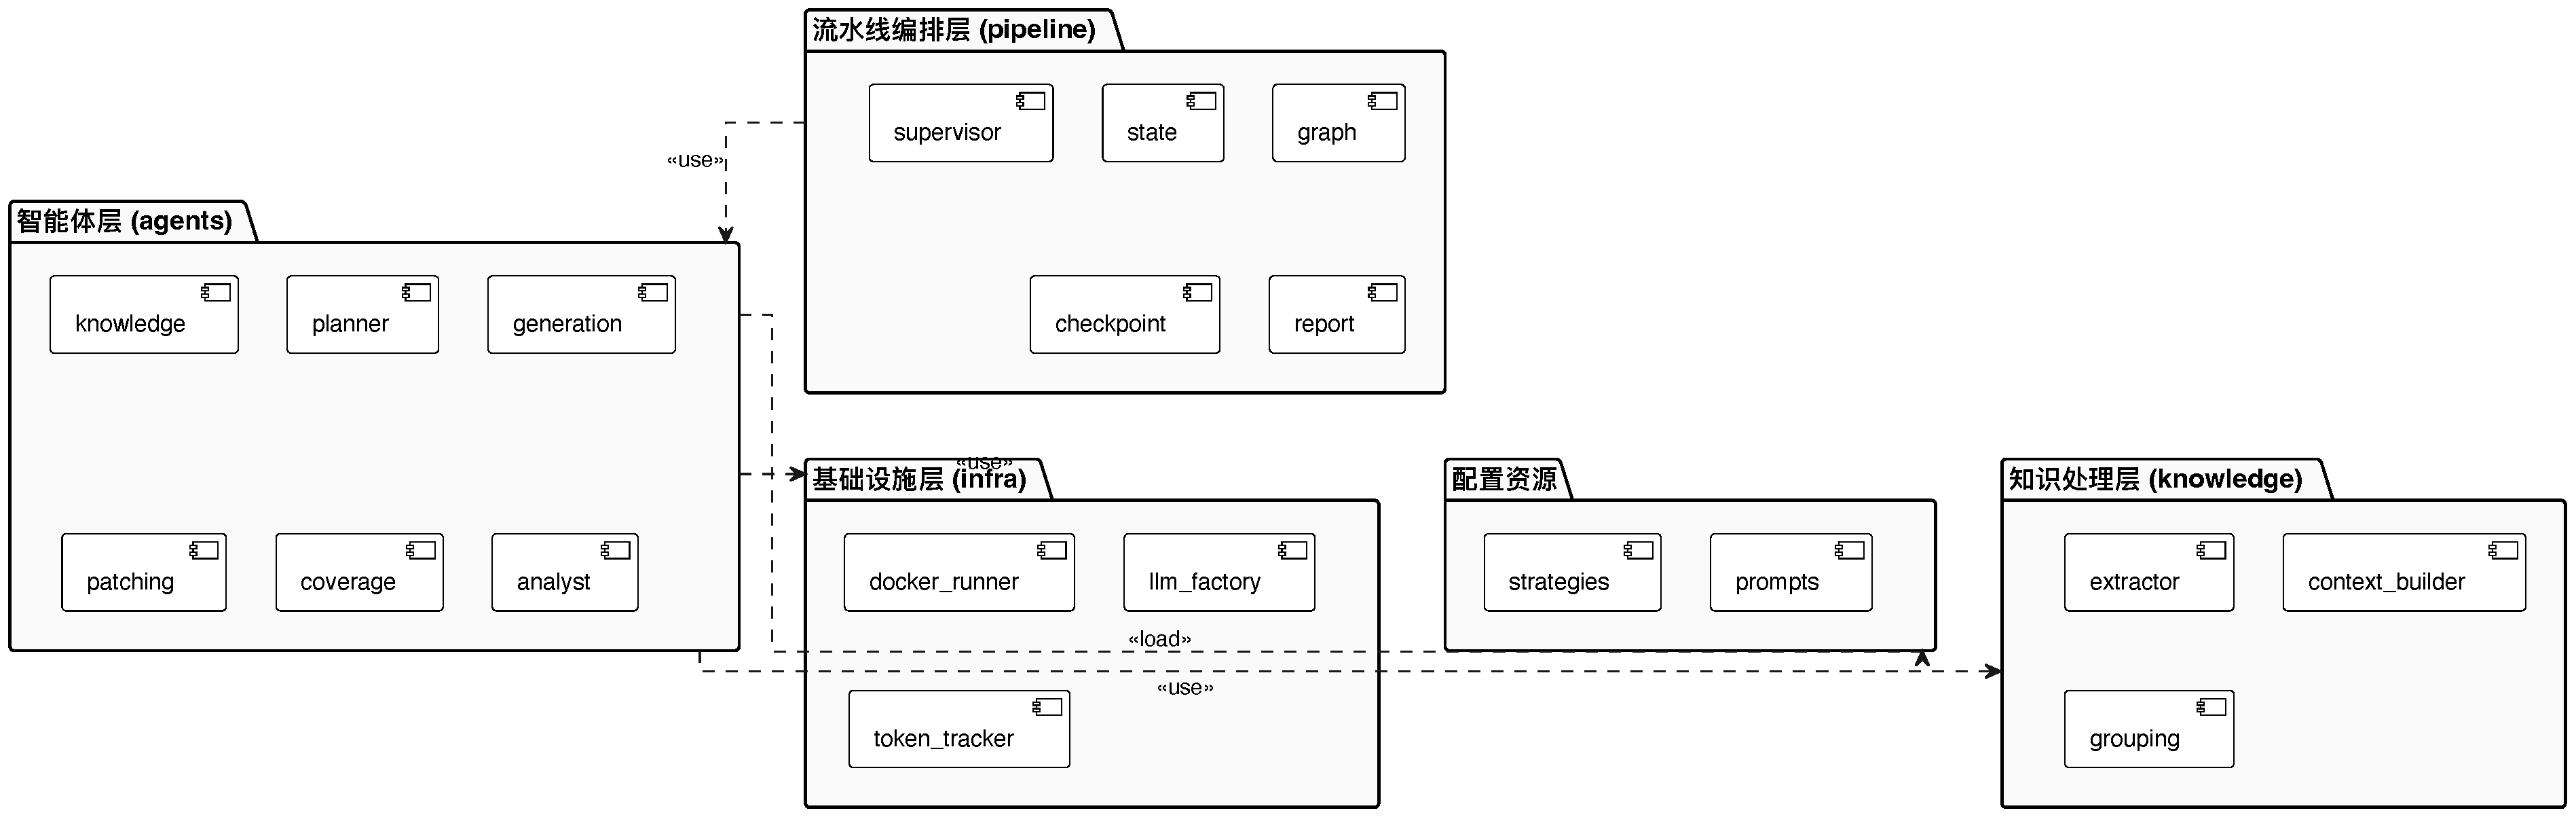
\includegraphics[width=1.2\textwidth]{images/development_view.pdf}}}
    \caption{MAGIC4FDG系统开发视图}
    \label{fig:dev-view}
\end{figure}

这个开发视图用包图展示了代码组织结构，面向开发人员设计。它遵循分层原则，自底向上分为四个代码层次：基础设施层、知识处理层、智能体层和流水线编排层。需要说明的是，代码层次划分是从软件工程的代码组织角度出发的，与3.3.2中按业务功能划分的七个模块存在映射关系：基础设施层对应基础设施模块，知识处理层对应知识处理模块，智能体层包含知识提取、策略规划与代码生成、编译修复、模糊测试与覆盖率收集、缺口诊断五个模块的实现，流水线编排层负责全局状态定义、DAG图构建、条件路由和检查点管理。

基础设施层（infra）包含docker\_runner、llm\_factory和token\_tracker三个包，分别封装Docker操作、LLM客户端创建和令牌统计。

知识处理层（knowledge）包含extractor、context\_builder和grouping三个包，分别负责AST JSON解析、按需格式化提示词文本、以及基于调用图的API分组和规则引擎策略匹配。

智能体层（agents）包含knowledge、planner、generation、patching、coverage和analyst六个包，每个包对应一个专职智能体，实现独立的节点函数，内部封装了提示词加载、LLM调用和结果解析的完整逻辑。

流水线编排层（pipeline）包含state、graph、supervisor、checkpoint和report五个包。state定义全局状态的TypedDict结构；graph构建LangGraph状态图并注册节点和条件路由；supervisor提供命令行入口和参数解析；checkpoint实现状态的JSON序列化与反序列化；report生成Markdown和JSON格式的实验报告。

另外还有两个辅助目录：strategies目录存储十种策略的Markdown文件（含YAML前置元数据），prompts目录存储各智能体的提示词模板。这两个目录作为配置资源，被智能体层在运行时动态加载。

\subsection{系统进程视图}

进程视图关注系统运行时的行为，描述并发性、进程间通信和同步机制。图\ref{fig:process-view}是MAGIC4FDG的进程视图。

\begin{figure}[H]
    \centering
    \makebox[\textwidth]{{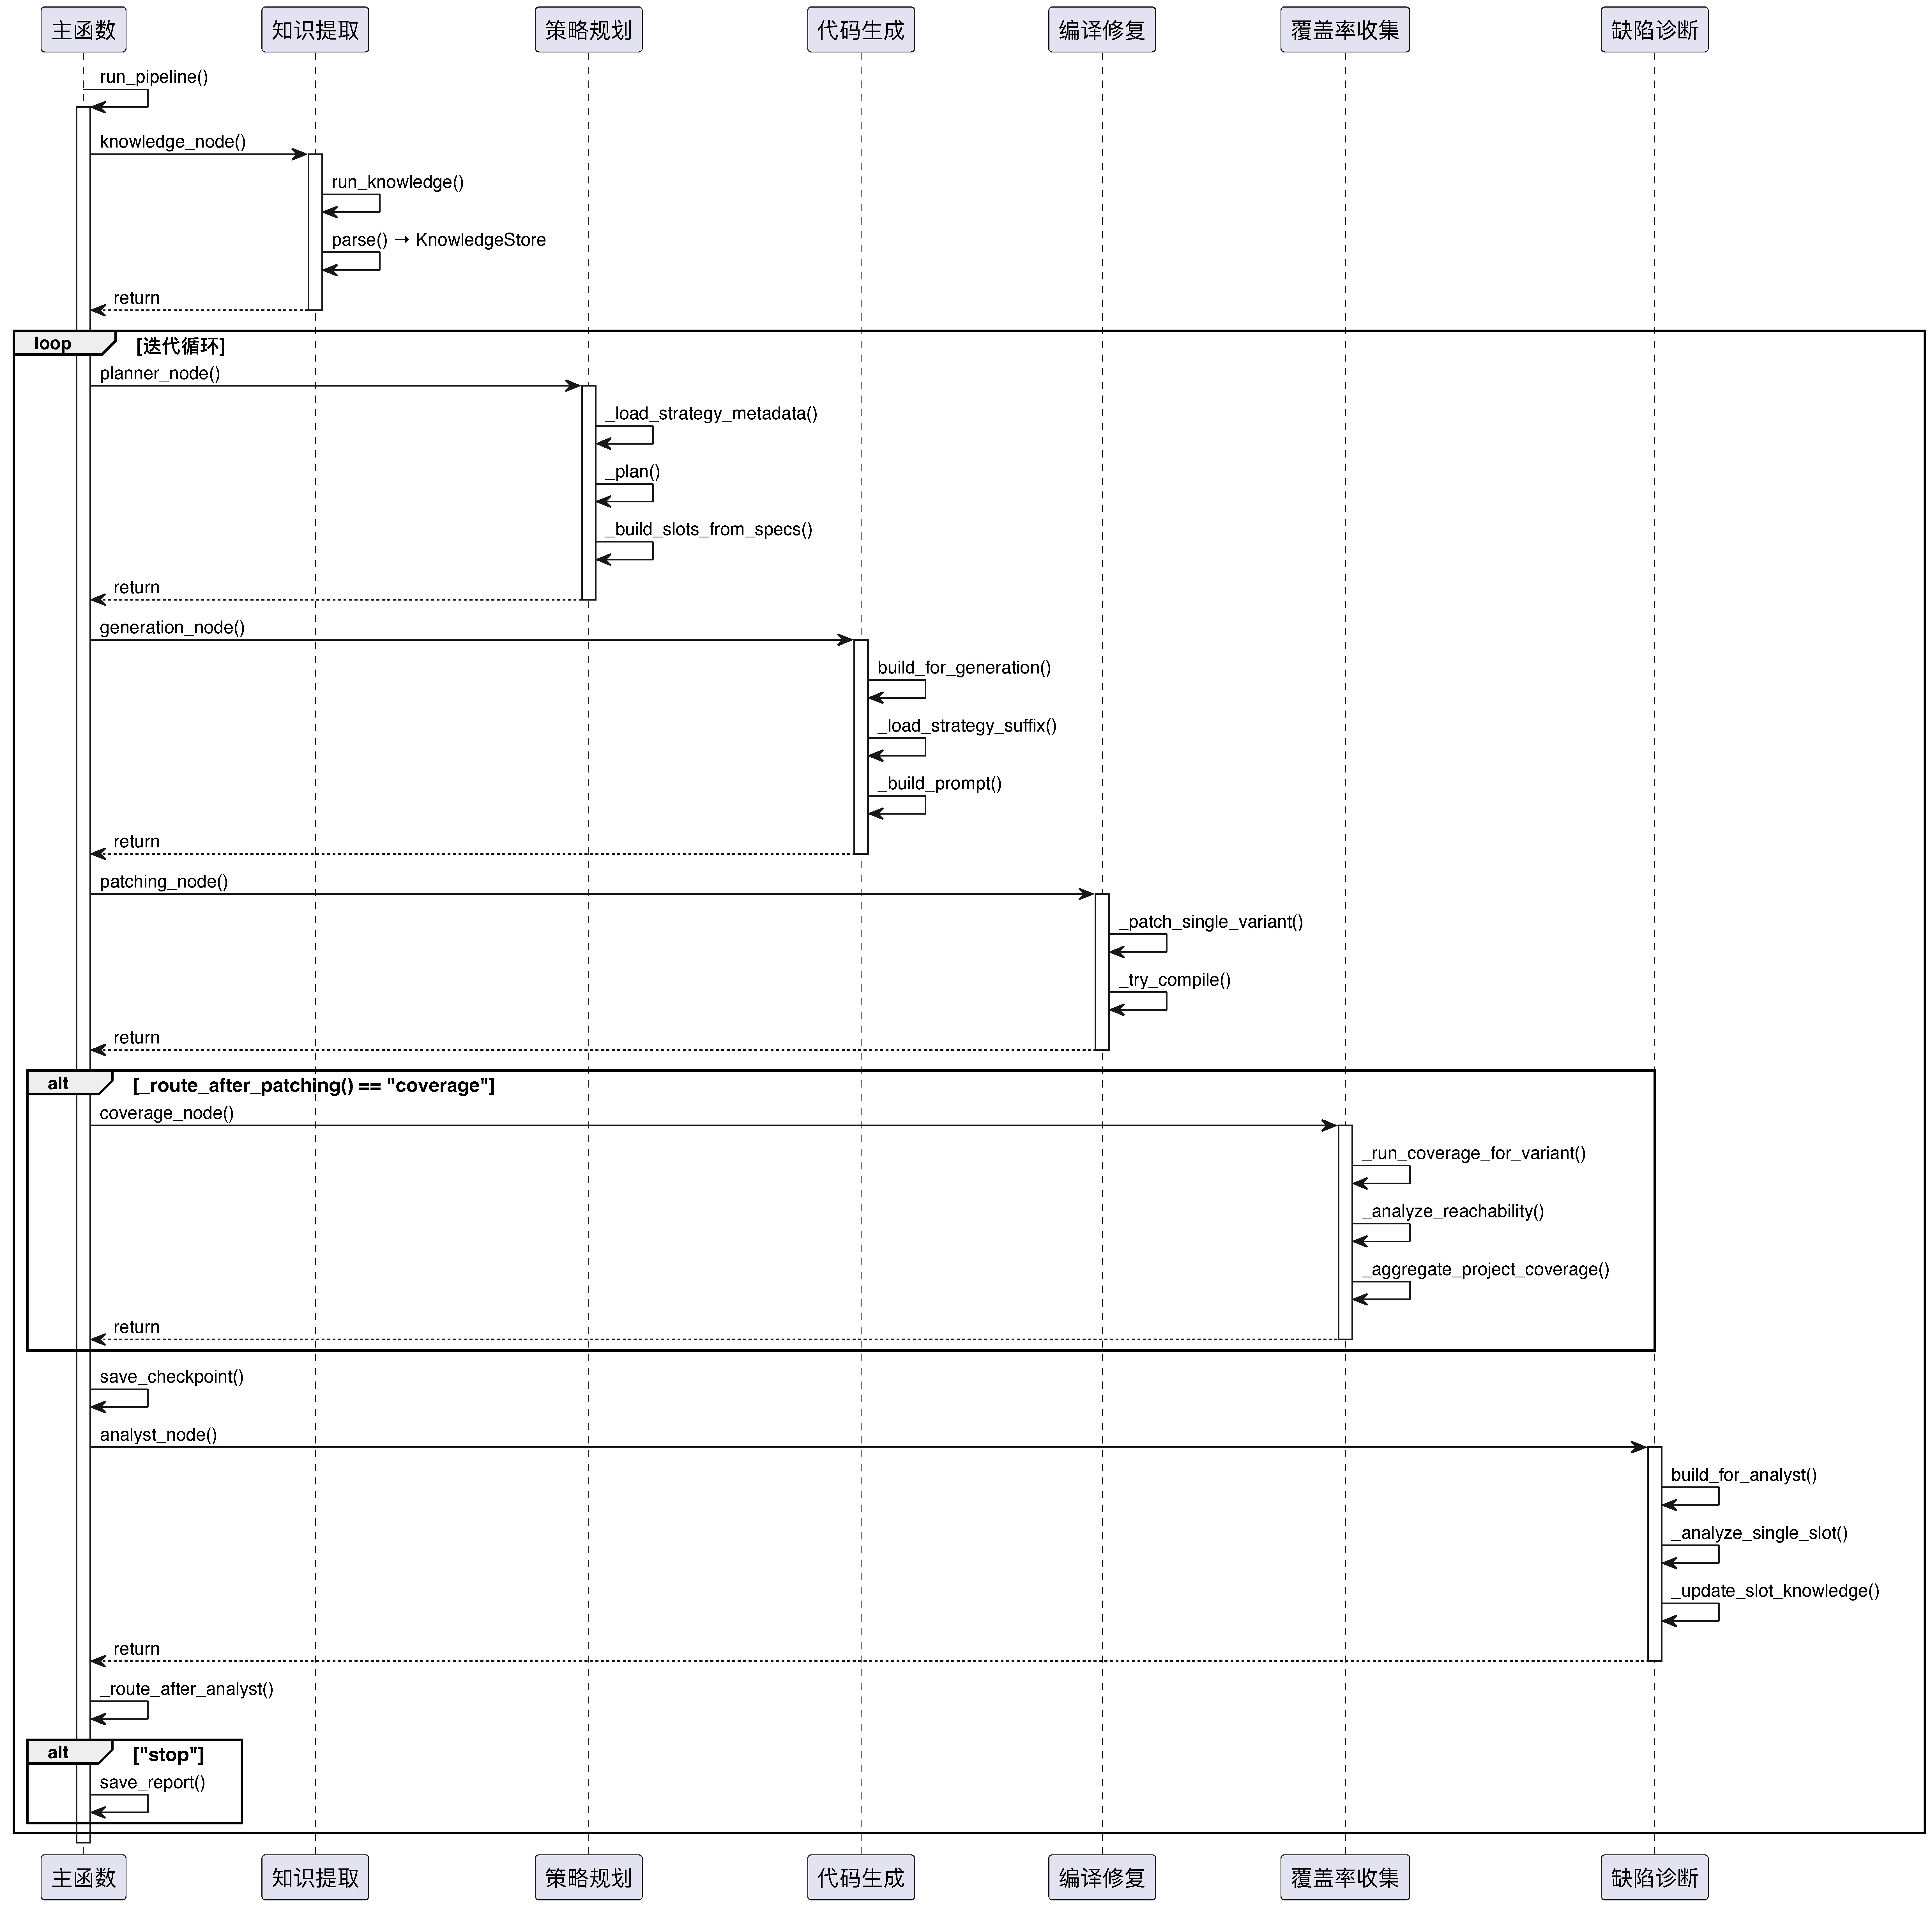
\includegraphics[width=1.1\textwidth]{images/seq_view.pdf}}}
    \caption{MAGIC4FDG系统进程视图}
    \label{fig:process-view}
\end{figure}

这个进程视图用顺序图展示系统运行时各组件的交互过程。重点展示事件触发和数据流转。系统共有八个组件在主函数的调度下协同工作：知识提取、知识处理、策略规划、代码生成、编译修复、覆盖率收集、状态持久化、缺口诊断。

主函数调用\texttt{run\_pipeline()}启动流水线后，先调用知识提取组件的\texttt{knowledge\_node()}。知识提取组件内部调用\texttt{run\_knowledge()}在Docker容器内编译目标库并做AST导出，再调用知识处理组件的\texttt{parse()}解析AST JSON，把结构化知识存入KnowledgeStore，构建产物缓存到宿主机。这一步只在首次运行时执行，后续通过检查缓存是否存在来决定是否跳过。

知识提取完成后进入迭代循环。每轮迭代中，主函数先调用策略规划组件的\texttt{planner\_node()}。该组件依次调用\texttt{\_load\_strategy\_metadata()}加载策略库元数据，首轮调用\texttt{\_plan\_initial()}通过LLM做API语义分析和策略匹配，后续轮次调用\texttt{\_plan\_iterate()}根据停滞计数调整策略，最后调用\texttt{\_build\_slots\_from\_specs()}构建槽位。

然后主函数调用代码生成组件的\texttt{generation\_node()}。该组件先调用知识处理组件的\texttt{build\_for\_generation()}获取格式化的API知识上下文，再调用\texttt{\_load\_strategy\_suffix()}加载策略后缀，最后根据轮次调用\texttt{\_build\_fresh\_prompt()}或\texttt{\_build\_incremental\_prompt()}组装提示词并调用LLM生成代码。

接着主函数调用编译修复组件的\texttt{patching\_node()}。该组件通过线程池对每个变体并行调用\texttt{\_patch\_single\_variant()}，内部调用\texttt{\_try\_compile()}在Docker容器内编译，失败的提取错误让LLM修复，最多三次。

编译修复完成后，主函数调用\texttt{\_route\_after\_patching()}做条件路由。有编译通过的变体就调用覆盖率收集组件的\texttt{coverage\_node()}，该组件通过线程池并行调用\texttt{\_run\_coverage\_for\_variant()}执行模糊测试和覆盖率收集，再调用\texttt{\_analyze\_reachability()}做CFG可达性分析，最后调用\texttt{\_aggregate\_project\_coverage()}算项目级覆盖率。全部编译失败则跳过直接进入下一步。

之后主函数调用状态持久化组件的\texttt{checkpoint\_node()}，内部调用\texttt{save\_checkpoint()}把流水线状态序列化为JSON检查点文件，同时保存各变体源码。

最后主函数调用缺口诊断组件的\texttt{analyst\_node()}。该组件先调用知识处理组件的\texttt{build\_for\_analyst()}获取未覆盖代码行的上下文，再通过线程池对每个活跃槽位并行调用\texttt{\_analyze\_single\_slot()}做根因分析，最后调用\texttt{\_update\_slot\_knowledge()}把结果追加到对应槽位的知识空间。

每轮迭代结束时，主函数调用\texttt{\_route\_after\_analyst()}检查终止条件（覆盖率达标、轮次上限、全部收敛、项目级停滞）。满足任一条件就调用\texttt{save\_report()}生成报告并终止；否则进入下一轮。

\subsection{系统物理视图}

物理视图关注部署架构，描述软件如何映射到硬件资源。图\ref{fig:deploy-view}是MAGIC4FDG的物理视图。

\begin{figure}[htbp]
    \centering
    \makebox[\textwidth]{{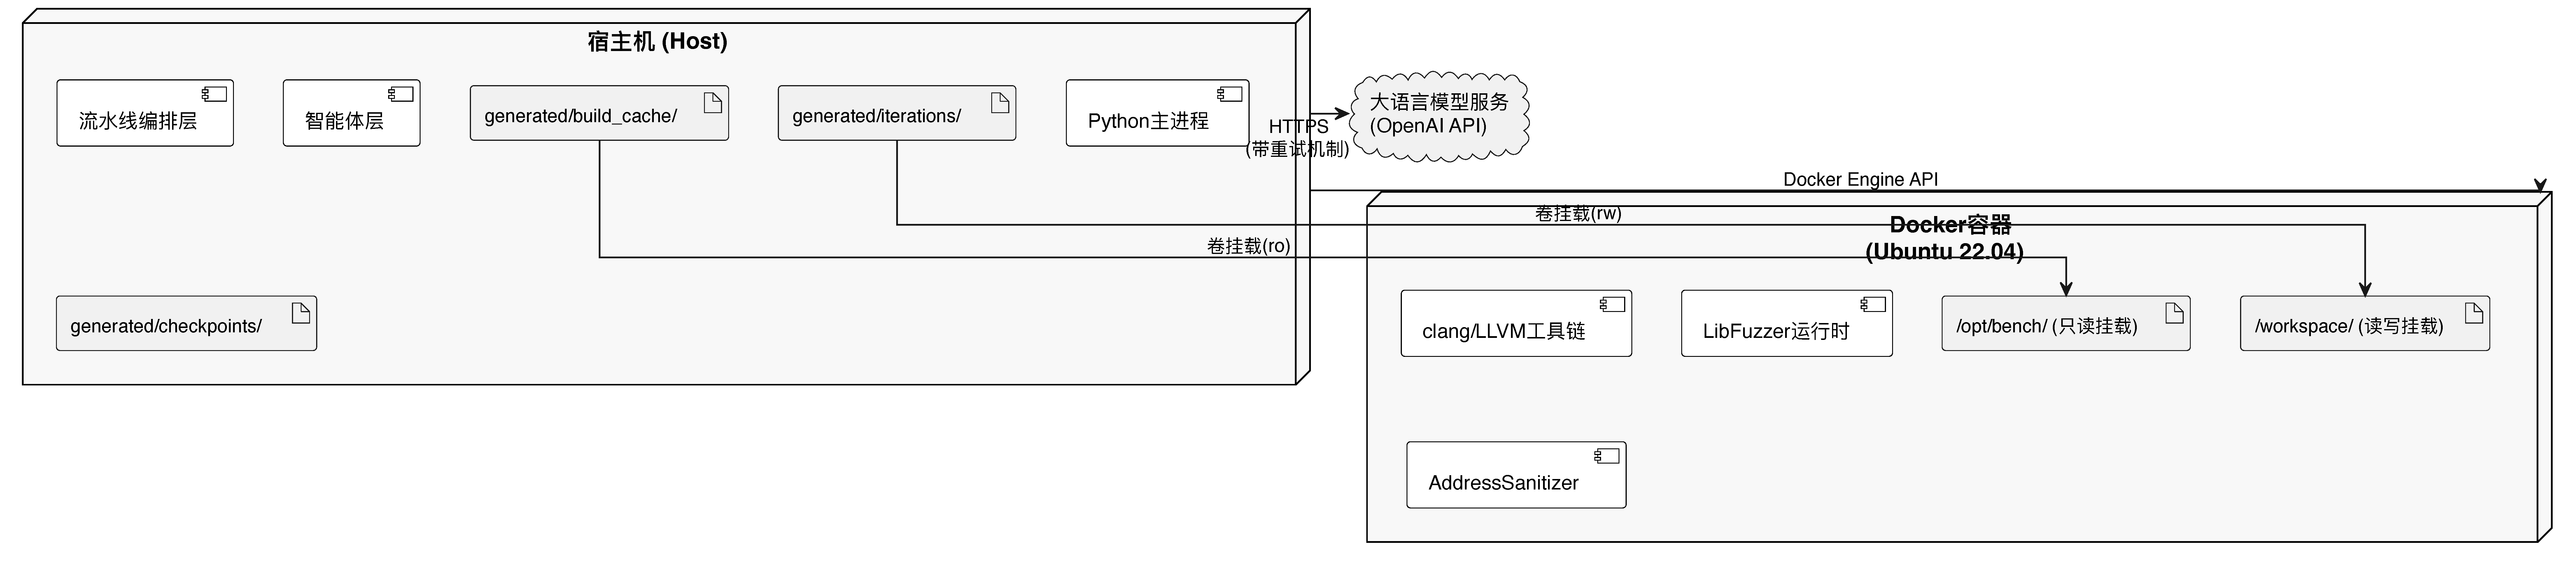
\includegraphics[width=\textwidth]{images/phy_view.drawio.pdf}}}
    \caption{MAGIC4FDG系统物理视图}
    \label{fig:deploy-view}
\end{figure}

部署结构分三块看：宿主机、Docker容器、LLM服务。

宿主机运行的是Python主进程，负责流水线编排和智能体调度。计算密集型操作（构建目标库、编译驱动、执行模糊测试、收集覆盖率）全部在Docker容器内完成。这一设计基于实际考虑——macOS上clang的行为与Linux不完全一致，直接在宿主机编译容易出现链接兼容性问题，因此统一使用Ubuntu 22.04容器，预装好clang/LLVM工具链和LibFuzzer。宿主机与容器之间通过卷挂载交换数据，构建缓存挂载为只读（/opt/bench），驱动源码和语料库通过读写卷双向传递。

LLM服务通过HTTPS调用，策略规划、代码生成、编译修复、缺口诊断四个环节都需要使用。本系统使用兼容OpenAI API格式的端点，配置文件中指定地址和密钥。考虑到网络波动，系统采用指数退避重试机制，实测中偶有超时但不会导致流水线中断。

\section{本章小结}

这一章完成了需求分析和概要设计，为后续的详细设计和编码实现提供了依据。

回顾一下本章内容。开头用流程图将系统运行的四个阶段阐述清楚，即知识准备、驱动生成与编译修复、模糊测试与覆盖率收集、缺口诊断与迭代控制，每个阶段中哪些智能体参与、如何配合都做了说明。

需求分析部分，本章梳理了三类涉众各自关心什么，再从中提炼出8项功能性需求和9项非功能性需求。用例分析画了用例图，选取了10个关键用例做了详细描述。用例描述较为详细，目的是为后续实现提供明确的验收标准。

概要设计部分，本章将系统划分为七个功能模块，分析了它们之间的数据依赖、功能依赖和状态依赖。然后用"4+1"视图从不同角度描述架构：逻辑视图描述类和依赖关系，开发视图描述代码组织与分层，进程视图描述运行时调用顺序和并行点，物理视图描述部署结构及三者间的通信方式。场景视图即前述用例图，此处不再赘述。